\section{線形回帰と最小二乗法}
\subsection{線形回帰}
$n$個のデータ $\left(y_1,x_{11}, \ldots x_{1p}\right),\ldots \left(y_n,x_{n1},\ldots, x_{np}\right)$ を説明変数$p$個の線形モデル 


\begin{equation}
y=\theta_0+\theta_1x_1+\cdots+\theta_px_p+\varepsilon=\theta_0+\sum_{j=1}^p \theta_jx_j+\varepsilon
\end{equation}


で説明することを考える (説明変数が単一の場合を単回帰,複数の場合を重回帰と呼ぶことがある).ここで, 


\begin{equation}
\mathbf{y}= \left[ \begin{array}{c} y_1\\ y_2\\ \vdots \\ y_n \end{array} \right],\quad 
\mathbf{X}=\left[ \begin{array}{ccccc} 1 & x_{11}& x_{12} &\cdots & x_{1p} \\ 1& x_{21}& x_{22}&\cdots & x_{2p}\\ \vdots & \vdots& \vdots& & \vdots \\1 &x_{n1} & x_{n2} &\cdots & x_{np} \end{array} \right],\quad
\mathbf{\theta}= \left[ \begin{array}{c} \theta_0\\ \theta_1\\ \vdots \\ \theta_p \end{array} \right]
\end{equation}


とすると,線形回帰モデルは $\mathbf{y}=\mathbf{X}\mathbf{\theta}+\mathbf{\varepsilon}$と書ける.ただし,$\mathbf{X}$は計画行列 (design matrix),$\mathbf{\varepsilon}$は誤差項である.特に,$\mathbf{\varepsilon}$が平均0, 分散$\sigma^2$の独立な正規分布に従う場合,$\mathbf{y}\sim \mathcal{N}(\mathbf{X}\mathbf{\theta}, \sigma^2\mathbf{I})$と表せる.
\subsection{最小二乗法によるパラメータの推定}
最小二乗法 (ordinary least squares)により線形回帰のパラメータを推定する.$y$の予測値は$\mathbf{X} \mathbf{\theta}$なので,誤差 $\mathbf{\delta} \in \mathbb{R}^n$は
$\mathbf{\delta} = \mathbf{y}-\mathbf{X} \mathbf{\theta}$と表せる.ゆえに目的関数$L(\mathbf{\theta})$は 


\begin{equation}
L(\theta)=\sum_{i=1}^n \delta_i^2 = \|\mathbf{\delta}\|^2=\mathbf{\delta}^\top \mathbf{\delta}
\end{equation}


となり, $L(\mathbf{\theta})$を最小化する$\mathbf{\theta}$, つまり $\hat {\mathbf {\theta }}={\underset {\mathbf {\theta}}{\operatorname {arg min} }}\,L({\mathbf{\theta}})$
を求める.
\subsubsection{勾配法を用いた推定}
最小二乗法による回帰直線を勾配法で求めてみよう.$\theta$の更新式は$\theta \leftarrow \theta + \alpha\cdot \dfrac{1}{n} \delta \mathbf{X}$と書ける.ただし,$\alpha$は学習率である.
\lstinputlisting[language=julia]{./text/introduction/linear-regression/003.jl}
\lstinputlisting[language=julia]{./text/introduction/linear-regression/004.jl}
\lstinputlisting[language=julia]{./text/introduction/linear-regression/005.jl}
\lstinputlisting[language=julia]{./text/introduction/linear-regression/006.jl}
\lstinputlisting[language=julia]{./text/introduction/linear-regression/007.jl}
\begin{figure}[ht]
	\centering
	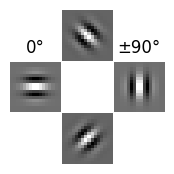
\includegraphics[scale=0.8, max width=\linewidth]{./fig/bayesian-brain/neural-sampling/cell007.png}
	\caption{cell007.png}
	\label{cell007.png}
\end{figure}
\subsubsection{正規方程式を用いた推定}
条件に基づいて目的関数$L(\mathbf{\theta})$を微分すると次のような方程式が得られる.


\begin{equation}
\mathbf{X}^\top\mathbf{X}\mathbf{\hat\theta}=\mathbf{X}^\top\mathbf{y}
\end{equation}


これを\textbf{\index{せいきほうていしき@正規方程式}} (normal equation)と呼ぶ.この正規方程式より、係数の推定値は$\mathbf{\hat\theta}={(\mathbf{X}^\top\mathbf{X})}^{-1}X^\top\mathbf{y}$という式で得られる.なお,正規方程式自体は$\mathbf{y}=\mathbf{X}\mathbf{\theta}$の左から$\mathbf{X}^\top$をかける,と覚えると良い.
\lstinputlisting[language=julia]{./text/introduction/linear-regression/009.jl}
\lstinputlisting[language=julia]{./text/introduction/linear-regression/010.jl}
\begin{figure}[ht]
	\centering
	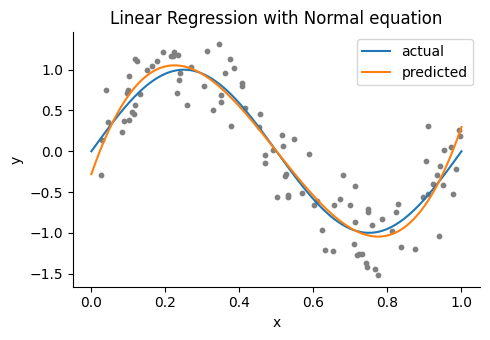
\includegraphics[scale=0.8, max width=\linewidth]{./fig/introduction/linear-regression/cell010.png}
	\caption{cell010.png}
	\label{cell010.png}
\end{figure}
